%\documentclass[journal ]{new-aiaa}
\documentclass[conf]{new-aiaa} % for conference papers
\usepackage[utf8]{inputenc}
\usepackage{textcomp}
\usepackage{listings}
\usepackage{graphicx}
\usepackage{amsmath}
\usepackage{caption,subcaption}
\usepackage[version=4]{mhchem}
\usepackage{siunitx}
\usepackage{multirow,longtable,tabularx}
\usepackage{float}
\usepackage[super]{nth}
\setlength\LTleft{0pt}

\title{Design and Analysis of Ram/Scramjet Engine}

\author{Stanley M. Porembski \footnote{Arizona State University Undergraduate Student, Aerospace Engineering (Autonomous Vehicle Systems).}}
\affil{Arizona State University Ira A. Schools of Engineering, Tempe, AZ, 85281}

\begin{document}

\maketitle

\begin{abstract}
The citation \cite{porembski2024github}.
\end{abstract}


\section*{Nomenclature}
{\renewcommand\arraystretch{1.0}
\noindent\begin{longtable*}{@{}l @{\quad=\quad} l@{}}
    $a_j$ & speed of sound for state $j$ \\
    $A$ & area \\
    $c_p$ & specific heat \\
    $M_j$ & mach number for state $j$ \\
    $p_j$ & static pressure for state $j$ \\
    $p_{tj}$ & total pressure for state $j$ \\
    $R$ & gas constant of air \\
    $s$ & specific entropy \\
    $T_j$ & static temperature for state $j$ \\
    $T_{tj}$ & total temperature for state $j$ \\
    $V_j$ & flow velocity for state $j$ \\
    $z$ & flight altitude \\
    $z^*$ & reference altitude \\
    $\eta$ & efficiency \\
    $\gamma$ & ratio of specific heats \\
\multicolumn{2}{@{}l}{Subscripts} \\
    1 & free stream conditions \\
    2 & inlet/diffuser conditions \\
    3 & combusor conditions \\
    e & nozzle flow conditions \\
    4 & external flow conditions \\
    s & conditions at Earth's surface
\end{longtable*}}


\section{Introduction} \label{sec:introduction}
\lettrine{T}{he} primary focus of this project was to develop an analysis tool for studies of non-ideal ramjet propulsion performance. This tool was developed using FORTRAN for the non-ideal ramjet propulsion system with a converging-only fixed-geometry nozzle in Fig.~\ref{fig:propsys}.

\begin{figure}[H] % Diagram of ram/scramjet propulsion system with state labels
    \centering
    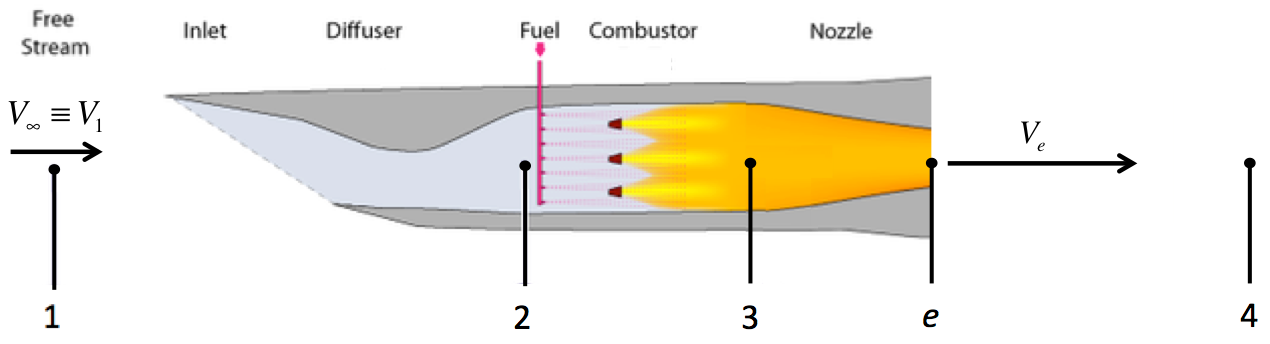
\includegraphics[width=0.75\textwidth]{media/the_ramjet.png}
    \caption{\label{fig:propsys} The Ramjet Propulsion System}
\end{figure}

To analyze the ramjet, the analysis tool was broken down into 5 modules focusing on an individual section of the flow path through the jet in Fig.~\ref{fig:propsys} and one module for calculating performance parameters. These modules take the given parameters listed in Table~\ref{tab:tool_inputs} along with the gas constant of air $R$, the ratio of specific heats $\gamma$, the gravitational acceleration $g$, and the specific heat $c_p$.

\begin{table}[H] % Table of Tool Inputs
    \caption{\label{tab:tool_inputs} Parametric Analysis Tool Inputs}
    \centering
    \begin{tabular}{lcc}
        \hline
        Name& Variable& Units\\\hline
        Flight Altitude& $z$& m\\
        Flight Mach Number& $M_1$\\
        Inlet/Diffuser Efficiency& $\eta_d$\\
        Combustor Inlet Mach Number& $M_2$\\
        Combustor Exit Max Allowable Total Temperature& $(T_{t3})_{max}$& K\\
        Chosen Fuel Heating Value& $q_f$& MJ/kg\\
        Nozzle Efficiency& $\eta_n$\\
        Nozzle Exit Area& $A_e$& $m^2$\\
        \hline
    \end{tabular}
\end{table}

Modules 1-5 calculate the properties listed in Table~\ref{tab:state_outputs} for each of the states shown in Fig.~\ref{fig:propsys}.

\begin{table}[H] % Table of State Outputs
    \caption{\label{tab:state_outputs} Parametric Analysis Tool State Outputs}
    \centering
    \begin{tabular}{llc}
        \hline
        Name& Variable& Units\\\hline
        Total Temperature& $T_{tj}$& K\\
        Static Temperature& $T_{j}$& K\\
        Total Pressure& $p_{tj}$& kPa\\
        Static Pressure& $p_j$& kPa\\
        Pressure Coefficient& $c_{pj}$& J/(kg-K)\\
        Flow Mach number& $M_j$\\
        Speed of Sound& $a_j$& m/s\\
        Flow Velocity& $V_j$& m/s\\
        Entropy Change from Previous State& $\Delta s_{(j-1),j}$& J/(kg-K)\\
        Relative Entropy& $\Delta s_{1,j}$& J/(kg-K)\\
        \hline
    \end{tabular}
\end{table}

These state properties are then used to calculate the performance parameters listed in Table~\ref{tab:perf_outputs}.

\begin{table}[H] % Table of Performance Outputs
    \caption{\label{tab:perf_outputs} Parametric Analysis Tool Performance Outputs}
    \centering
    \begin{tabular}{llc}
        \hline
        Name& Variable& Units\\\hline
        Heat per Unit Mass Added in the Combustor& $q_{23}$& MJ/kg\\
        Nozzle Exit Mass Flux& $\dot m_e$& kg/s\\
        Inlet Mass Flux& $\dot m_i$& kg/s\\
        Fuel Mass Flux& $\dot m_f$& kg/s\\
        Fuel-Air Mass Ratio& $f$\\
        Jet Thrust& $T_{jet}$& N\\
        Pressure Thrust& $T_{pressure}$& N\\
        Total Thrust& $T_{total}$& N\\
        Equivalent Velocity& $V_{eq}$& m/s\\
        Thrust Specific Fuel Consumption& $TSFC$& (kg/hr)/N\\
        Specific Impulse& $I_{sp}$& s\\
        Thermal Efficiency& $\eta_{th}$\\
        Propulsive Efficiency& $\eta_p$\\
        Overall Efficiency& $\eta_o$\\
        Propulsive Power& $P$& W\\
        \hline
    \end{tabular}
\end{table}

The analysis tool was then used by iterating the inputs to observe how the performance parameters of the ram/scramjet vary. After analyzing trends, the tool was used to design two propulsion systems that optimize different performance parameters.


\section{Theory} \label{sec:theory}
The ram/scramjet is "basically one of the most simple types of aircraft engine," consisting of an inlet/diffuser, a combustion system, and an exit nozzle. The system primarily produces thrust through ram action requiring the engine to be moving to create thrust, so zero thrust is produced at zero flight speed. Aircraft utilizing ram/scramjet propulsion systems will also need another method of propulsion to boost the speed of the aircraft close to Mach 1 before the ramjet system produces a usable amount of thrust. \cite{nasa1956ramjetperformance}.

The ram/scramjet operates on the Brayton cycle. Oncoming airflow is compressed by the inlet/diffuser through ram compression. The kinetic energy of the air is converted to pressure energy as it passes through the diffuser \cite{rycey1996jetengine}. The pressure increase is dependent on the isentropic efficiency of the diffuser. For ramjets, the flow speed of the oncoming air is slowed to under Mach 0.4, while Scramjets are defined by the Mach entering the combustor being supersonic.

The airflow then has liquid fuel injected into it before entering the combustion chamber. The liquid fuel needs to be atomized, vaporized, and mixed in with the airflow before the combustion process occurs \cite{oates1997aerothermodynamics}.

The combustor adds heat to the fuel-air mixture through combustion to increase the temperature of the mixture to the thermal limits of the engine materials. When adding heat in the combustor it is necessary to determine if the combustor will be thermally choked. Thermal choking occurs when the heat addition for the Mach entering the combustor is so large that no combination of thermodynamic and flow conditions can absorb the heat. The only solution is for the Mach entering the combustor to be reduced to accommodate the added heat such that the Mach leaving the combustor $M_3=1$. This is accomplished by unstarting the inlet of the ramjet where a normal shock forms in front of the inlet to reduce the free stream Mach which will reduce the Mach entering the combustor \cite{dahm2023project}. Any further fuel that is injected into the combustor to increase the temperature past the choked temperature will be wasted.

The exiting flow from the combustor then travels through the converging-only nozzle. In the converging nozzle, subsonic flow will be sped up and supersonic flow will be slowed down. The supersonic flow will be slowed down to Mach 1 at the smallest cross section of the converging nozzle and if subsonic flow is accelerated enough it reach its maximum speed of Mach 1 in the throat of the nozzle. This phenomenon is known as nozzle choking.

The fuel-air mixture leaving a non-choked nozzle will be at ambient air temperature. When leaving a choked nozzle, the gas mixture will not be at ambient air temperatures and will travel through expansion, compression, and shock waves to equalize its pressure with the surrounding air. This process is highly irreversible.

The gas at ambient pressure then equalizes with the surrounding air to complete the Brayton cycle.


\section{Tool Calculations} \label{sec:tool_calculations}
\subsection{State 1: Free Stream}
The properties of the free stream entering the propulsion system were modeled using the isentropic model of the atmosphere. This was split into two sections, properties for altitudes under 7958 meters and properties above 7958 meters. For altitudes $z<7958$ m, Eq.~\eqref{eqn:T1_low} and Eq.~\eqref{eqn:p1_low} were used with $T_s=288$ K, $p_s=101.3$ kPa, $\gamma=1.4$, and $z^*=8404$ m to find the static temperature $T_1$ and static pressure $p_1$ of state 1. $\gamma$ was taken as 1.4.

\begin{equation}
    \label{eqn:T1_low}
    \frac{T_1}{T_s}\equiv\frac{T(z)}{T_s}=\left[1-\frac{\gamma-1}{\gamma}(z/z^*)\right]
\end{equation}

\begin{equation}
    \label{eqn:p1_low}
    \frac{p_1}{p_s}\equiv\frac{p(z)}{p_s}=\left[1-\frac{\gamma-1}{\gamma}(z/z^*)\right]^\frac{\gamma}{\gamma-1}
\end{equation}

For altitudes $z>7958$ m, $T_1\equiv T(z)=$ constant = 210 K while the static pressure was solved for using,

\begin{equation}
    \label{eqn:p1_high}
    p_1\equiv p(z)=33.6e^{-\left[\frac{z-7958}{6605}\right]}
\end{equation}

With the calculated $T_1$ and $p_1$ and the inputted flight Mach number $M_1$, the total temperature $T_{t1}$ and pressure $p_{t1}$ were calculated from the total-to-static relations for temperature using Eq.~\eqref{eqn:Tt1} and pressure using Eq.~\eqref{eqn:pt1}.

\begin{equation}
    \label{eqn:Tt1}
    \frac{T_{t1}}{T_1}=\left[1+\frac{\gamma-1}{2}M_1^2\right]
\end{equation}

\begin{equation}
    \label{eqn:pt1}
    \frac{p_{t1}}{p_1}=\left[1+\frac{\gamma-1}{2}M_1^2\right]^\frac{\gamma}{\gamma-1}
\end{equation}

After calculating the total and static temperature and pressure of state 1, the speed of sound $a_1$ and flight speed $V_1$ were calculated. $R$ was taken as 286.9 J/(kg-K).

\begin{equation}
    \label{eqn:a1}
    a_1=\sqrt{\gamma RT_1}
\end{equation}

\begin{equation}
    \label{eqn:V1}
    V_1=M_1\cdot a_1
\end{equation}

\subsection{State 2: Inlet/Diffuser}
The inlet/diffuser of the ramjet engine does not do work on nor take work out of the oncoming air. It also does not transfer any heat into or out of the air, so the total temperature at state two is,

\begin{equation}
    \label{eqn:Tt2}
    T_{t2}=T_{t1}
\end{equation}

Then with the total temperature calculated, the given combustor inlet Mach number $M_2$ was used to calculate the static temperature using the total-to-static relation,

\begin{equation}
    \label{eqn:T2}
    \frac{T_{t2}}{T_2}=\left[1+\frac{\gamma-1}{2}M_2^2\right]
\end{equation}

The speed of sound and the flow speed entering the combustor could then be calculated from the computed state 2 static temperature using Eq.~\eqref{eqn:a2} and Eq.~\eqref{eqn:V2}, respectively.

\begin{equation}
    \label{eqn:a2}
    a_2=\sqrt{\gamma R T_2}
\end{equation}

\begin{equation}
    \label{eqn:V2}
    V_2=M_2\cdot a_2
\end{equation}

To obtain the total pressure at state 2, the free stream Mach number $M_1$ and the given inlet/diffuser isentropic efficiency $\eta_d$ were used in the following equation.

\begin{equation}
    \label{eqn:pt2}
    \frac{p_{t2}}{p_1}=\left[1+\eta_d\frac{\gamma-1}{2}M_1^2\right]^{\frac{\gamma}{\gamma-1}}
\end{equation}

With the total pressure at state 2 calculated, the static pressure was calculated from the total-to-static relation,

\begin{equation}
    \label{eqn:p2}
    \frac{p_{t2}}{p_2}=\left[1+\frac{\gamma-1}{2}M_2^2\right]^{\frac{\gamma}{\gamma-1}}
\end{equation}

With the total temperature and pressure calculated, the entropy increase from the sources of irreversibility in the inlet/diffuser flow was calculated using the Second Law as,

\begin{equation}
    \label{eqn:dels12}
    \Delta s_{12}\equiv \left(s_2-s_1\right)=\left(s_{t2}-s_{t1}\right)=c_p \ln\frac{T_{t2}}{T_{t1}}-R\ln\frac{p_{t2}}{p_{t1}}
\end{equation}

where $c_p$ was calculated using,

\begin{equation}
    \label{eqn:cp}
    c_p=\frac{\gamma R}{\gamma-1}
\end{equation}

\subsection{State 3: Combustor}
From this state onwards, $\gamma=1.3$ due to the addition of fuel into the airflow. To determine the Mach number $M_3$ and the total temperature $T_{t3}$, it was first required to determine if the combustor was thermally choked. The choked total temperature $\left(T_{t3}\right)_{choked}$ was calculated by setting $M_3=1$ and using,

\begin{equation}
    \label{eqn:Tt3choked}
    \left(T_{t3}\right)_{choked}=T_{t2}\cdot\left\{\frac{1}{2(\gamma+1)}\cdot\frac{1}{M_2^2}\left(1+\gamma M_2^2\right)^2\left(1+\frac{\gamma-1}{2}M_2^2\right)^{-1}\right\}
\end{equation}

The calculated value of the choked total temperature was then compared against the given max temperature $\left(T_{t3}\right)_{max}=2400K$. If $\left(T_{t3}\right)_{choked}\leq\left(T_{t3}\right)_{max}$, then $M_3=1$ and $T_{t3}=\left(T_{t3}\right)_{choked}$. However, if $\left(T_{t3}\right)_{choked}>\left(T_{t3}\right)_{max}$, then $T_{t3}=\left(T_{t3}\right)_{max}$ and $M_3$ was calculated by rearranging Eq.~\eqref{eqn:Tt3/Tt2} into a quadratic equation in terms of $\left(M_3^2\right)$.

\begin{equation}
    \label{eqn:Tt3/Tt2}
    \frac{T_{t3}}{T_{t2}}=\frac{M_3^2}{M_2^2}\cdot\frac{\left(1+\gamma M_2^2\right)^2}{\left(1+\gamma M_3^2\right)^2}\cdot\frac{\left(1+\frac{\gamma-1}{2}M_3^2\right)}{\left(1+\frac{\gamma-1}{2}M_2^2\right)}
\end{equation}

First, the constant,

\begin{equation}
    \label{eqn:C}
    C\equiv\frac{T_{t3}}{T_{t2}}\cdot\frac{\left(1+\frac{\gamma-1}{2}M_2^2\right)}{\left(1+\gamma M_2^2\right)^2}M_2^2=\frac{\left(1+\frac{\gamma-1}{2}M_3^2\right)}{\left(1+\gamma M_3^2\right)^2}M_3^2
\end{equation}

then Eq.~\eqref{eqn:Tt3/Tt2} was rearranged into the quadratic form of,

\begin{equation}
    \label{eqn:quad}
    \underbrace{\left[C\gamma^2-\frac{\gamma-1}{2}\right]}_\text{a}
    \left(M_3^2\right)^2+
    \underbrace{\left[2C\gamma-1\right]}_\text{b}
    \left(M_3^2\right)+
    \underbrace{C}_\text{c}
    =0
\end{equation}

and the constants used to solve for $M_3$.

\begin{equation}
    \label{eqn:quadeq}
    \left(M_3^2\right)=\frac{-b\pm\sqrt{b^2-4ac}}{2a}
\end{equation}

The only roots that were selected from the quadratic equation were those where $\left(M_3^2\right)>0$. Then if $M_2<1$ then $M_3>M_2$ and $M_3\leq1$, and if $M_2>1$ then $M_3<M_2$ and $M_3\geq1$. The heat per unit mass $q_{23}$ that was added in the combustor was calculated using Eq.~\eqref{eqn:q23}.

\begin{equation}
    \label{eqn:q23}
    q_{23}=\int_{T_{t2}}^{T_{t3}} c_p(T) \,dT=a\left[T_{t3}-T_{t2}\right]+\frac{1}{2}b\left[T_{t3}^2-T_{t2}^2\right]
\end{equation}

The specific heat model,

\begin{equation}
    \label{eqn:latercp}
    c_p (T)=a+bT
\end{equation}

was used for calculating the specific heat in Eq.~\eqref{eqn:q23} where $(a,b)=(986,0179)$. From the calculated Mach number, the static temperature $T_3$ and the total pressure $p_{t3}$ were calculated using their respective total-to-static relations.

\begin{equation}
    \label{eqn:T3}
    \frac{T_{t3}}{T_3}=\left[1+\frac{\gamma-1}{2}M_3^2\right]
\end{equation}

\begin{equation}
    \label{eqn:pt3}
    \frac{p_{t3}}{p_3}=\left[1+\frac{\gamma-1}{2}M_3^2\right]^\frac{\gamma}{\gamma-1}
\end{equation}

Since the combustor operates at constant pressure,

\begin{equation}
    \label{eqn:p3}
    p_3=p_2
\end{equation}

Then the speed of sound and flow velocity were calculated.

\begin{equation}
    \label{eqn:a3}
    a_3=\sqrt{\gamma RT_3}
\end{equation}

\begin{equation}
    \label{eqn:V3}
    V_3=M_3\cdot a_3
\end{equation}

The entropy increase across the combustor was calculated using Eq.~\eqref{eqn:latercp} as,

\begin{equation}
    \label{eqn:dels23}
    \Delta s_{23}\equiv\left(s_3-s_2\right)=\left(s_{t3}-s_{t2}\right)=c_p\ln\frac{T_{t3}}{T_{t2}}-R\ln\frac{p_{t3}}{p_{t2}}
\end{equation}

Then the relative entropy was calculated as,

\begin{equation}
    \label{eqn:dels13}
    \Delta s_{13}=(s_3-s_1)=\Delta s_{12}+\Delta s_{23}
\end{equation}

\subsection{State e: Internal Converging Nozzle Flow}
For the internal flow in the converging nozzle, seen in Fig.~\ref{fig:propsys}, it was first necessary to see if the exit flow of the nozzle is choked. First, the test Mach number was calculated using,

\begin{equation}
    \label{eqn:M'}
    M'\equiv\left\{\frac{2}{\gamma-1}\cdot\frac{\eta_n\left[1-\left(p_1/p_{t3}\right)^{\frac{\gamma-1}{\gamma}}\right]}{1-\eta_n\left[1-\left(p_1/p_{t3}\right)^{\frac{\gamma-1}{\gamma}}\right]}\right\}^{1/2}
\end{equation}

From the test Mach number, the state of the nozzle could be determined. If $M'<1$ then the nozzle is not choked and the exit Mach and static pressure could be calculated as,

\begin{equation}
    \label{eqn:nchokeMe}
    M_e=M'
\end{equation}

and,

\begin{equation}
    \label{eqn:nchokepe}
    p_e=p_1
\end{equation}

However, if $M'\geq1$ then the nozzle flow is choked and the exit Mach and static pressure could instead be calculated as,

\begin{equation}
    \label{eqn:chokeMe}
    M_e=1
\end{equation}

and,

\begin{equation}
    \label{eqn:chokepe}
    p_e=p_{t3}\left[1-\frac{1}{\eta_n}\left(\frac{\gamma-1}{\gamma+1}\right)\right]^\frac{\gamma}{\gamma-1}
\end{equation}

The nozzle does not do work on or have work done on it by the gas nor does it transfer any heat between the gas, so by the \nth{1} Law,

\begin{equation}
    \label{eqn:Tte}
    T_{te}=T_{t3}
\end{equation}

Then the static temperature and the total pressure for the nozzle exit were calculated using the total-to-static relations,

\begin{equation}
    \label{eqn:Te}
    \frac{T_{te}}{T_e}=\left[1+\frac{\gamma-1}{2}M_e^2\right]
\end{equation}

\begin{equation}
    \label{eqn:pte}
    \frac{p_{te}}{p_e}=\left[1+\frac{\gamma-1}{2}M_e^2\right]^\frac{\gamma}{\gamma-1}
\end{equation}

With the total and static properties at the nozzle's exit, the speed of sound and flow velocity were found with,

\begin{equation}
    \label{eqn:ae}
    a_e=\sqrt{\gamma R T_e}
\end{equation}

\begin{equation}
    \label{eqn:Ve}
    V_e=M_e\cdot a_e
\end{equation}

The exit mass flux of the nozzle was calculated using,

\begin{equation}
    \label{eqn:mdote}
    \dot{m}_e=\rho_e V_e A_e=\frac{p_e}{R T_e}V_e A_e
\end{equation}

The entropy increase from the nozzle irreversibilities was calculated using,

\begin{equation}
    \label{eqn:dels3e}
    \Delta s_{3e}\equiv\left(s_e-s_3\right)=\left(s_{te}-s_{t3}\right)=c_p \ln\frac{T_{te}}{T_{t3}}-R\ln\frac{p_{te}}{p_{t3}}
\end{equation}

where $c_p$ was calculated using Eq.~\eqref{eqn:latercp} for the exit temperature $T_e$. This entropy increase was then used to calculate the relative entropy with,

\begin{equation}
    \label{eqn:dels1e}
    \Delta s_{1e}=s_e-s_1=\Delta s_{12}+\Delta s_{23}+\Delta s_{3e}
\end{equation}

\subsection{State 4: External Flow Past Nozzle Exit}
The pressure of the ambient air was taken as,

\begin{equation}
    \label{eqn:p4}
    p_4=p_1
\end{equation}

Depending on the choked state of the converging only, the external nozzle flow efficiency could be calculated from the test Mach number that was calculated using Eq.~\eqref{eqn:M'} as

\begin{equation}
    \label{eqn:eta_n_ext}
    \eta_{n,ext} = \begin{cases}
        1 & \text{if } M' \leq 1 \\
        M'^{-0.3} & \text{if } M' \geq 1 \\
    \end{cases}
\end{equation}

Again, from the \nth{1} Law, there is no work or heat transfer interactions with the gas, so

\begin{equation}
    \label{eqn:Tt4}
    T_{t4}=T_{te}=T_{t3}
\end{equation}

Then using $\gamma=1.3$, the static temperature of the gas leaving the nozzle was calculated using,

\begin{equation}
    \label{eqn:T4}
    \frac{T_4}{T_{te}}=1-\eta_{n,ext}\left[1-\left(p_1/p_{te}\right)^\frac{\gamma-1}{\gamma}\right]
\end{equation}

With the total and static temperature, the Mach number could be calculated for state 4 by rearranging the total-to-static relation for state 4 to,

\begin{equation}
    \label{eqn:M4}
    M_4=\left\{\frac{2}{\gamma-1}\left[\frac{T_{t4}}{T_4}-1\right]\right\}^{1/2}
\end{equation}

Then with the Mach number, the total pressure of state 4 was calculated from the total-to-static pressure relations,

\begin{equation}
    \label{eqn:pt4}
    \frac{p_{t4}}{p_4}=\left[1+\frac{\gamma-1}{2}M_4^2\right]^\frac{\gamma}{\gamma-1}
\end{equation}

The speed of sound and flow velocity were calculated as,

\begin{equation}
    \label{eqn:a4}
    a_4=\sqrt{\gamma R T_4}
\end{equation}

and,

\begin{equation}
    \label{eqn:V4}
    V_4=M_4\cdot a_4
\end{equation}

Lastly, the entropy increase due to the irreversibility in the external nozzle flow was calculated as,

\begin{equation}
    \label{eqn:delse4}
    \Delta s_{e4}\equiv(s_4-s_e)=(s_{t4}-s_{te})=c_p \ln\frac{T_{t4}}{T_{te}}-R\ln\frac{p_{t4}}{p_{te}}
\end{equation}

where $c_p$ is calculated from Eq.~\eqref{eqn:latercp} and the relative entropy was calculated using,

\begin{equation}
    \label{eqn:dels14}
    \Delta s_{14}=(s_4-s_1)=\Delta s_{12}+\Delta s_{23}+\Delta s_{3e}+\Delta s_{e4}
\end{equation}

\subsection{Ram/Scramjet Performance Parameters}
The inlet mass flux was calculated using $q_{23}$ calculated from Eq.~\eqref{eqn:q23}, $\dot{m}_e$ calculated from Eq.~\eqref{eqn:mdote}, and the given $q_f$ using,

\begin{equation}
    \label{eqn:mdoti}
    \left. \dot{m}_i=\dot{m}_e \middle/ \left(1+\frac{q_{23}}{q_f}\right) \right.
\end{equation}

which was then used to calculate the fuel mass flux from,

\begin{equation}
    \label{eqn:mdotf}
    \dot{m}_f=\dot{m}_e-\dot{m}_i
\end{equation}

then used to compute the fuel-air mass ratio $f$ using Eq.~\eqref{eqn:f}.

\begin{equation}
    \label{eqn:f}
    \left. f\equiv\dot{m}_f\middle/\dot{m}_i \right.
\end{equation}

The jet, pressure, and total thrust $T$ were then calculated using $p_\infty\equiv p_1$ and $V_\infty\equiv V_1$ from Module 1, $p_e$ and $V_e$ calculated from Module 4, and the given nozzle exit area $A_e$ using,

\begin{equation}
    \label{eqn:Thrust}
    T=
    \underbrace{\dot{m}_i\left[\left(1+f\right)V_e-V_1\right]}_\text{Jet thrust}
    +
    \underbrace{\left(p_e-p_1\right)A_e}_\text{Pressure thrust}
\end{equation}

The thrust-specific fuel consumption was then calculated with,

\begin{equation}
    \label{eqn:TSFC}
    TSFC=\frac{\dot{m}_f}{T}
\end{equation}

and converted to units of $(kg/hr)/N$. The specific impulse was then computed in units of seconds using $g=9.8$ m/s\textsuperscript{2} with,

\begin{equation}
    \label{eqn:Isp}
    I_{sp}=\frac{T}{\dot{m}_f g}
\end{equation}

To then compute the thermal efficiency, the equivalent velocity $V_{eq}$ that would produce the same thrust $T$ if the nozzle exit flow were fully expanded was first calculated as,

\begin{equation}
    \label{eqn:Veq}
    V_{eq}=V_e+\left(p_e-p_\infty\right)\frac{A_e}{\dot{m}_e}
\end{equation}

With $V_{eq}$ the thermal efficiency was calculated with,

\begin{equation}
    \label{eqn:etath}
    \eta_{th}=\frac{\left[\dot{m}_e\frac{1}{2}V_{eq}^2\right]-\left[\dot{m}_i\frac{1}{2}V_{1}^2\right]}{\dot{m}_i q_{23}}
\end{equation}

The propulsive efficiency $\eta_{p}$ was then calculated from the equivalent velocity as,

\begin{equation}
    \label{eqn:etap}
    \left. \eta_p=\frac{2}{1+\left(V_{eq}\middle/V_1\right)} \right.
\end{equation}

and used to calculate the overall efficiency as,

\begin{equation}
    \label{eqn:etao}
    \eta_o=\eta_{th}\cdot\eta_p
\end{equation}

Lastly, the propulsive power was calculated with,

\begin{equation}
    \label{eqn:P}
    P=T\cdot V_\infty
\end{equation}


\section{Ram/Scramjet Analysis Procedures} \label{sec:ram_scramjet_analysis_procedures}
The analysis tool created from the calculations in section \ref{sec:tool_calculations} was validated using two test cases: Case A for the non-thermally choked test case and Case B for the thermally choked test case. The inputs of each case for the analysis tool are listed in Table \ref{tab:val_case_input}. Between the two cases, it can be seen that the only difference between them is the value of $M_2$, the Mach entering the combustion chamber. The outputs of the analysis tool were compared to the expected case outputs listed in Table \ref{tab:val_case_output}. With the analysis tool validated, the inputs to the tool were modified and iterated to analyze ram/scramjet performance. The performance analysis was broken down into nine sections with plots provided to visualize the parameter's variability.

\subsection{\textit{T-s} Diagrams for Validation Cases} % Part A
Using the validation inputs for Case A and B, \textit{T-s} diagrams were created for each case using the computed static temperature and entropy change values. For the interconnecting lines between each state, straight lines were used between states 1 and 2, 3 and e, and e and 4. Constant pressure curves were used between states 2 and 3 and states 4 and 1. The constant pressure curve for 2-3 was defined as,

\begin{equation}
    \label{eqn:constp_23}
    \left(\frac{dT}{ds}\right)_p=\frac{T}{c_p} \quad \rightarrow \quad dT=\frac{T}{a+bT}ds
\end{equation}

since the specific heat was defined using Eq. \ref{eqn:latercp} for this section. The constant pressure curve for 4-1 was defined as,

\begin{equation}
    \label{eqn:constp_41}
    \left(\frac{dT}{ds}\right)_p=\frac{T}{c_p} \quad \rightarrow \quad dT=\frac{T}{c_p}ds
\end{equation}

since $c_p$ was taken as a constant value of 1004 J/kg-K.

\subsection{Atmospheric Model Validation} % Part B
The isentropic atmosphere model used in module 1 for calculating the static temperature and pressure of the free stream entering the ram/scramjet was compared to the tabulated ICAO Standard Atmosphere \cite{hill1992propulsion}.

\subsection{Effect of Flight Mach Number} % Part C
The flight Mach number was iterated from $0.8\leq M_1\leq 5.0$ using the other input parameters from the unchoked validation case A. The overall efficiency $\eta_o$, thrust $T_{total}$, and TSFC were analyzed against the varied flight Mach number to determine its effect on the parameters.

\subsection{Effect of Flight Altitude} % Part D
The flight altitude was iterated from $2 km \leq z \leq 30 km$ using the other input parameters from the unchoked validation case A. This variability was analyzed to determine how $\eta_o$, $T_{total}$, and TSFC are affected.

\subsection{Optimizing TSFC} % Part E
The input parameters from the unchoked validation case A were used while iterating $2 km \leq z \leq 20 km$ in steps of 500 m. For each of these flight altitude values the flight Mach number $M_1$ was iterated to find the values that would maximize $\eta_o$ and minimize the TSFC.

\subsection{Effect of Inlet/Diffuser Efficiency} % Part F
Using the input parameters from validation case A with $z=4300m$ and $M_1=2.4$, the inlet/diffuser efficiency was iterated from $0.5\leq\eta_d\leq1.0$ in steps of 0.05. The resulting $\eta_o$, $T_{total}$, and TSFC that are calculated were analyzed against the varied inlet/diffuser efficiency.

\subsection{Effect of Nozzle Efficiency} % Part G
Using the input parameters from case A with $z=4300m$ and $M_1=2.4$, the nozzle efficiency was iterated from $0.5\leq\eta_n\leq1.0$ in steps of 0.05. The variation of the nozzle efficiency was compared against the calculated $\eta_o$, $T_{total}$, and TSFC.

\subsection{Effect of \texorpdfstring{\textit{$M_2$}}{M2}} % Part H
The input parameters from case A were used with $z=4300m$ and $M_1=2.4$ and the combustor inlet Mach number $M_2$ was varied from $0.1\leq M_2\leq2.5$ in steps of 0.1 to calculate $\eta_o$, $T_{total}$, and TSFC. The effect of the combustor inlet Mach on the three performance parameters was analyzed.

\subsection{Optimized Ram/Scramjet Propulsion System} % Part I
The parametric analysis tool was used to design a ram/scramjet propulsion system for hypersonic flight at $M_1=5$ and $z=90,000ft$ (27,400 m) with the same fuel heating value $q_f$ and inlet/diffuser and nozzle efficiencies as in case A and the combustor exit total temperature was limited to $\left(T_{t3}\right)_{max}\leq2400K$. The combustor inlet Mach $M_2$ and the combustor exit total temperature $T_{t3}$ were iterated to find two sets of parameters that would maximize the thrust and that would maximize the overall efficiency.


\section{Results} \label{sec:results}
\subsection{\textit{T-s} Diagrams for Validation Cases} % Part A
The \textit{T-s} diagrams for cases A and B are plotted in Figure \ref{fig:partavalida} and Figure \ref{fig:partavalidb} respectively. It can be seen that the entropy from state 1-2 and state 3-4 increases which was expected from the given isentropic efficiencies of the inlet/diffuser and nozzle.

The area contained within the plots is proportional to the net work generated by the engine. It can be seen that the non-thermally choked case A encloses a larger area than the thermally choked case B. This behavior is expected as for the thermally choked case the temperature of state 3 is limited which puts a limit on the size of the \textit{T-s} diagram and the net work from the ramjet.

\begin{figure}[H] % Part A: T-s diagram for validation case A
    \centering
    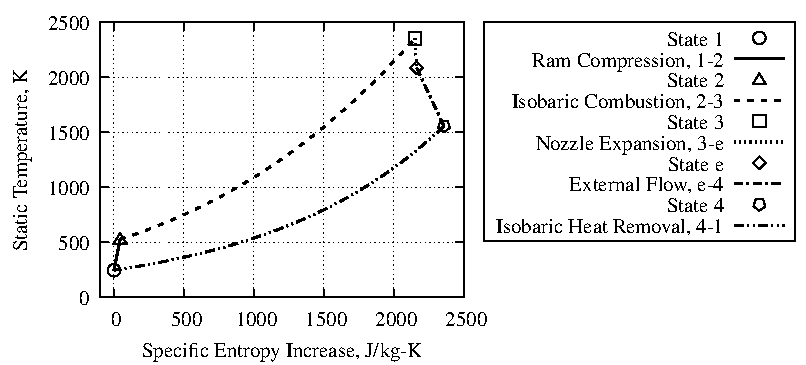
\includegraphics[]{media/ts_plot_files/TS_plot_for_case_7.pdf}
    \caption{\label{fig:partavalida}Validation Case A}
\end{figure}

\begin{figure}[H] % Part A: T-s diagram for validation case B
    \centering
    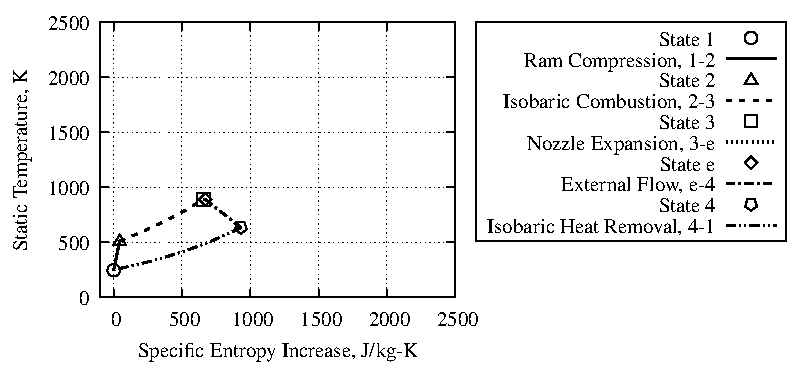
\includegraphics[]{media/ts_plot_files/TS_plot_for_case_8.pdf}
    \caption{\label{fig:partavalidb}Validation Case B}
\end{figure}

\subsection{Atmospheric Model Validation} % Part B
When comparing the isentropic atmosphere model to the ICAO standard atmosphere it can be seen that the pressure readings seen in Fig. \ref{fig:partbpres} match each other closely with the isentropic model underestimating the pressure slightly. So, the isentropic model is a sufficient model of the pressure distribution of the atmosphere.

\begin{figure}[H] % Part B: Atmosphere Validation comparing Isen to ICAO: Pressure
    \centering
    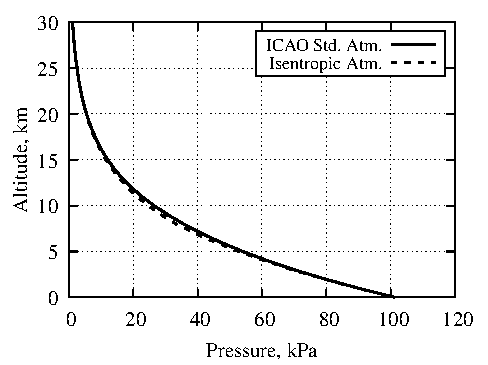
\includegraphics[]{media/atmosphere_validation_files/ICAO_vs_ISEN_pressure.pdf}
    \caption{\label{fig:partbpres}ICAO Standard Atmosphere vs Isentropic Model (Pressure)}
\end{figure}

However, it can be seen in Fig. \ref{fig:partbtemp} that the temperature readings from the isentropic atmosphere model vary significantly from the ICAO standard atmosphere. When comparing the 1\% temperature extremes \cite{nasa1976standardatmos} to the isentropic model it can be seen that, for the altitude range of interest, the isentropic model lies within the temperature limits. Since the model is within the variability of the atmosphere, it is acceptable to use for the atmosphere's temperature variability in the ram/scramjet analysis.

\begin{figure}[H] % Part B: Atmosphere Validation comparing Isen to ICAO: Temperature
    \centering
    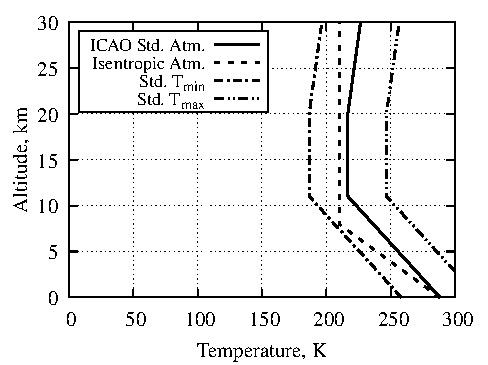
\includegraphics[]{media/atmosphere_validation_files/ICAO_vs_ISEN_temperature.pdf}
    \caption{\label{fig:partbtemp}ICAO Standard Atmosphere vs Isentropic Model (Temperature)}
\end{figure}

\subsection{Effect of Flight Mach Number} % Part C

% \begin{figure}[H] % Part C: total temperature for varied flight Mach
%     \centering
%     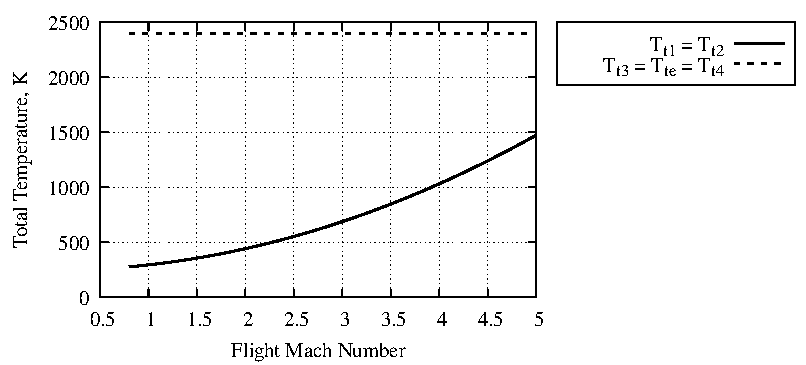
\includegraphics[]{media/performance_parameter_files/part_c_total_temperature.pdf}
%     \caption{\label{fig:partctotaltemperature}Total Temperature vs Flight Mach Number}
% \end{figure}

\subsubsection{Overall Efficiency}
The relation between the overall efficiency and the flight Mach number can be seen in Fig. \ref{fig:partcetao}. It can be seen that increasing the flight Mach number leads to an increase in $\eta_o$ rising to a maximum value of $\eta_o\approx0.275$ at $M_1\approx3.25$. After this value, the overall efficiency rapidly decreases as the Mach increases.

\begin{figure}[H] % Part C: overall efficiency for varied flight Mach
    \centering
    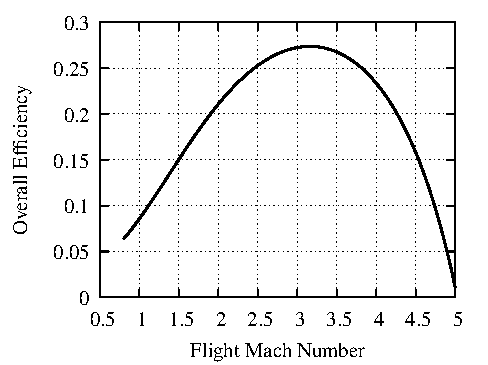
\includegraphics[]{media/performance_parameter_files/part_c_eta_o.pdf}
    \caption{\label{fig:partcetao}Overall Efficiency vs Flight Mach Number}
\end{figure}

The overall efficiency is comprised of the propulsive and thermal efficiency seen in Eq. \ref{eqn:etao}. From the velocity plot in Fig. \ref{fig:partcvelocity}, it can be seen using Eq. \ref{eqn:etap} that the propulsive efficiency will increase with the Mach number reaching an efficiency of 1 at $M_1=5$ since $V_{eq}=V_1$. 

\begin{figure}[H] % Part C: velocity for varied flight Mach
    \centering
    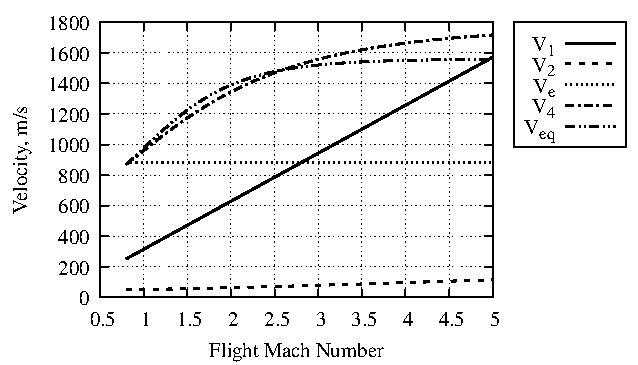
\includegraphics[]{media/performance_parameter_files/part_c_velocity.pdf}
    \caption{\label{fig:partcvelocity}Velocity vs Flight Mach Number}
\end{figure}

This means that the thermal efficiency must be what causes the overall efficiency to decrease after $M_1\approx3.25$. Rearranging Eq. \ref{eqn:etath} by canceling out like terms gives,

\begin{equation}
    \label{eqn:partcetath}
    \eta_{th}=\frac{\frac{1}{2}\left[(1+f)V_{eq}^2-V_1^2\right]}{q_{23}}
\end{equation}

where the fuel-air mass ratio $f\approx0.06$ at $M_1=0.8$ and decreases to $f\approx0.03$ at $M_1=5$. 

\subsubsection{Total Thrust}
The

\begin{figure}[H] % Part C: total thrust for varied flight Mach
    \centering
    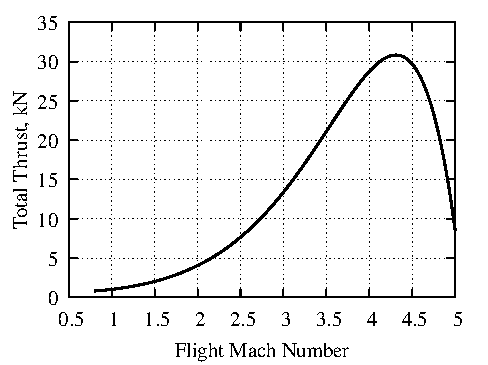
\includegraphics[]{media/performance_parameter_files/part_c_T.pdf}
    \caption{\label{fig:partct}Total Thrust vs Flight Mach Number}
\end{figure}
The

\subsubsection{Thrust Specific Fuel Consumption}
The

\begin{figure}[H] % Part C: TSFC for varied flight Mach
    \centering
    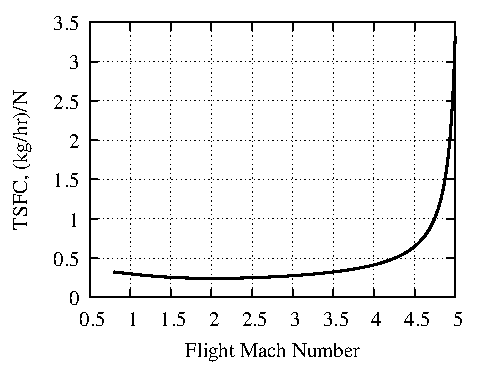
\includegraphics[]{media/performance_parameter_files/part_c_TSFC.pdf}
    \caption{\label{fig:partctsfc}TSFC vs Flight Mach Number}
\end{figure}
The

\subsection{Effect of Flight Altitude} % Part D
The

\subsubsection{Overall Efficiency}
The

\begin{figure}[H] % Part D: overall efficiency for varied flight altitude
    \centering
    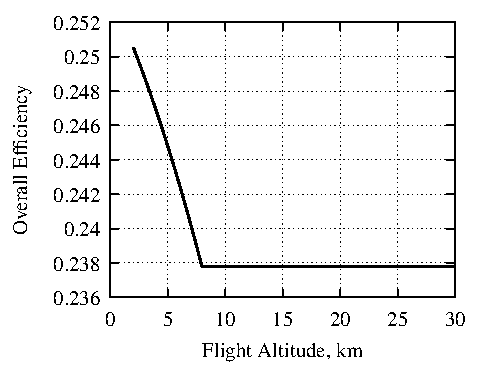
\includegraphics[]{media/performance_parameter_files/part_d_eta_o.pdf}
    \caption{\label{fig:partdetao}Overall Efficiency vs Flight Altitude}
\end{figure}
The

\subsubsection{Total Thrust}
The

\begin{figure}[H] % Part D: total thrust for varied flight altitude
    \centering
    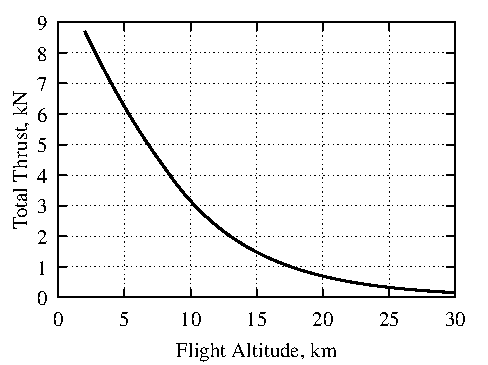
\includegraphics[]{media/performance_parameter_files/part_d_T.pdf}
    \caption{\label{fig:partdt}Total Thrust vs Flight Altitude}
\end{figure}
The

\subsubsection{Thrust Specific Fuel Consumption}
The

\begin{figure}[H] % Part D: TSFC for varied flight altitude
    \centering
    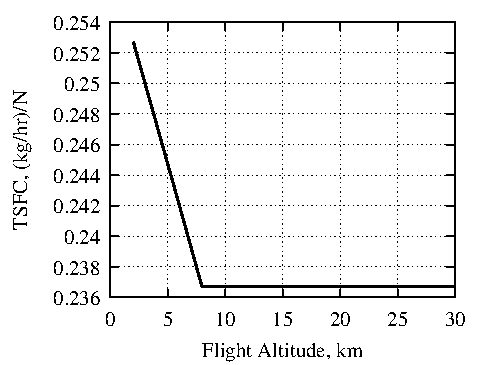
\includegraphics[]{media/performance_parameter_files/part_d_TSFC.pdf}
    \caption{\label{fig:partdtsfc}TSFC vs Flight Altitude}
\end{figure}
The

\subsection{Optimizing TSFC} % Part E
The

\begin{figure}[H] % Part E: optimize overall efficiency and TSFC for varied flight altitude with Mach 1-5
    \centering
    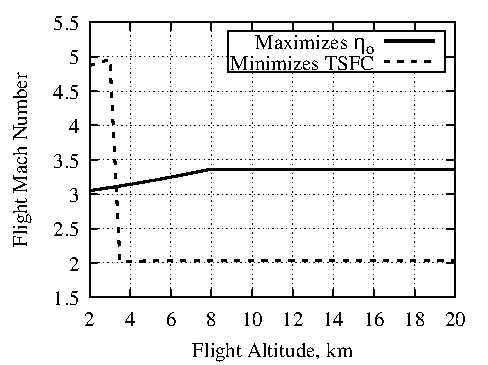
\includegraphics[]{media/performance_parameter_files/part_e_range_1_5.pdf}
    \caption{\label{fig:parte1-5}Optimizing Overall Efficiency and TSFC, Mach 1-5}
\end{figure}

\begin{figure}[H] % Part E: optimize overall efficiency and TSFC for varied flight altitude with Mach 1-10
    \centering
    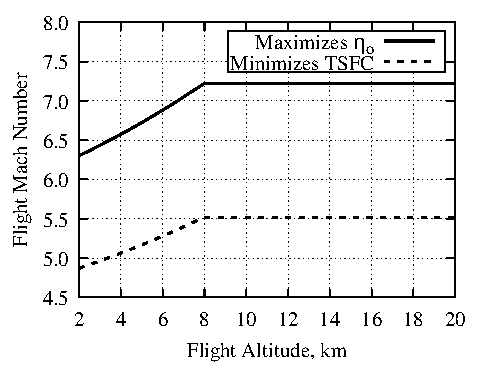
\includegraphics[]{media/performance_parameter_files/part_e_range_1_10.pdf}
    \caption{\label{fig:parte1-10}Optimizing Overall Efficiency and TSFC, Mach 1-10}
\end{figure}

\subsection{Effect of Inlet/Diffuser Efficiency} % Part F
The

\subsubsection{Overall Efficiency}
The

\begin{figure}[H] % Part F: overall efficiency for varied inlet/diffuser efficiency
    \centering
    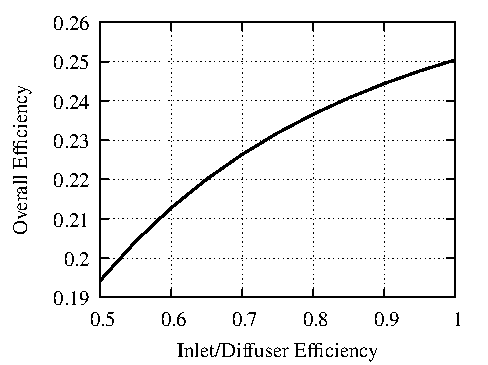
\includegraphics[]{media/performance_parameter_files/part_f_eta_o.pdf}
    \caption{\label{fig:partfetao}Overall Efficiency vs Inlet/Diffuser Efficiency}
\end{figure}
The

\subsubsection{Total Thrust}
The

\begin{figure}[H] % Part F: total thrust for varied inlet/diffuser efficiency
    \centering
    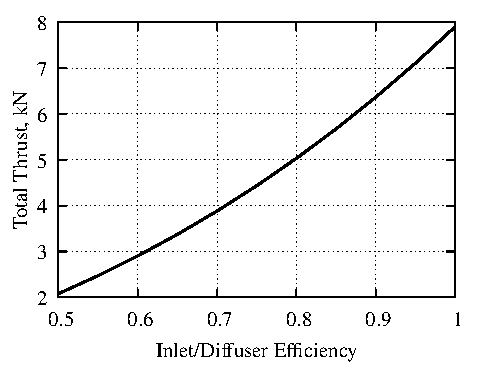
\includegraphics[]{media/performance_parameter_files/part_f_T.pdf}
    \caption{\label{fig:partft}Total Thrust vs Inlet/Diffuser Efficiency}
\end{figure}
The

\subsubsection{Thrust Specific Fuel Consumption}
The

\begin{figure}[H] % Part F: TSFC for varied inlet/diffuser efficiency
    \centering
    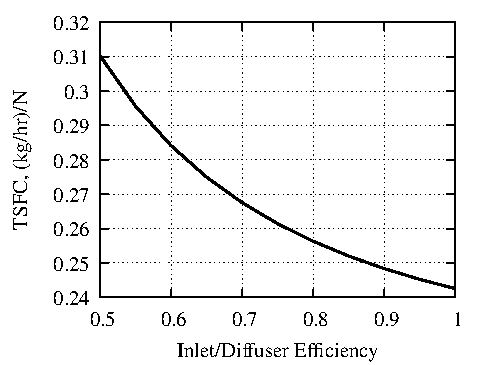
\includegraphics[]{media/performance_parameter_files/part_f_TSFC.pdf}
    \caption{\label{fig:partftsfc}TSFC vs Inlet/Diffuser Efficiency}
\end{figure}
The

\subsection{Effect of Nozzle Efficiency} % Part G
The

\subsubsection{Overall Efficiency}
The

\begin{figure}[H] % Part G: overall efficiency for varied nozzle efficiency
    \centering
    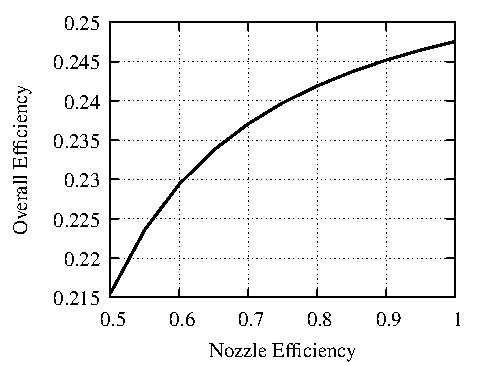
\includegraphics[]{media/performance_parameter_files/part_g_eta_o.pdf}
    \caption{\label{fig:partgetao}Overall Efficiency vs Nozzle Efficiency}
\end{figure}
The

\subsubsection{Total Thrust}
The

\begin{figure}[H] % Part G: total thrust for varied nozzle efficiency
    \centering
    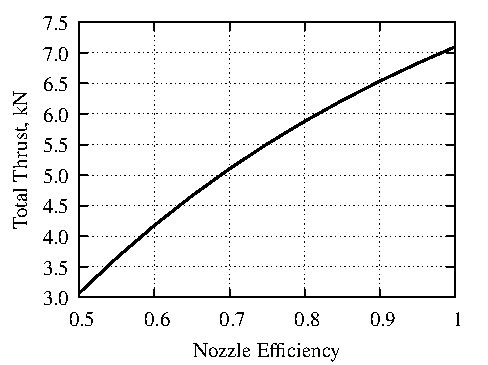
\includegraphics[]{media/performance_parameter_files/part_g_T.pdf}
    \caption{\label{fig:partgt}Total Thrust vs Nozzle Efficiency}
\end{figure}
The

\subsubsection{Thrust Specific Fuel Consumption}
The

\begin{figure}[H] % Part G: TSFC for varied nozzle efficiency
    \centering
    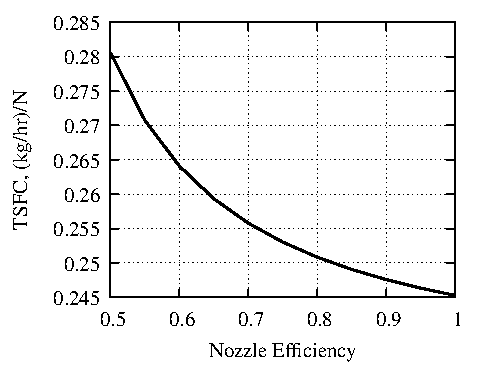
\includegraphics[]{media/performance_parameter_files/part_g_TSFC.pdf}
    \caption{\label{fig:partgtsfc}TSFC vs Nozzle Efficiency}
\end{figure}
The

\subsection{Effect of \texorpdfstring{\textit{$M_2$}}{M2}} % Part H
The

\subsubsection{Overall Efficiency}
The

\begin{figure}[H] % Part H: overall efficiency for varied combustor Mach
    \centering
    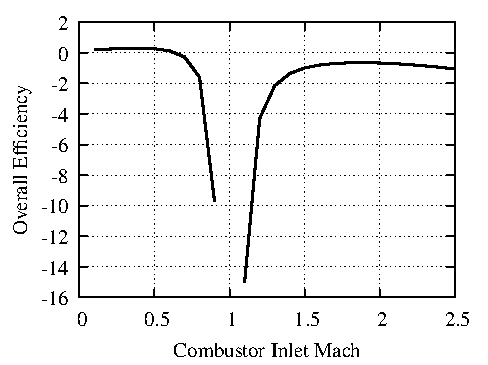
\includegraphics[]{media/performance_parameter_files/part_h_eta_o.pdf}
    \caption{\label{fig:parthetao}Overall Efficiency vs \texorpdfstring{\textit{$M_2$}}{M2}}
\end{figure}
The

\subsubsection{Total Thrust}
The

\begin{figure}[H] % Part H: total thrust for varied combustor Mach
    \centering
    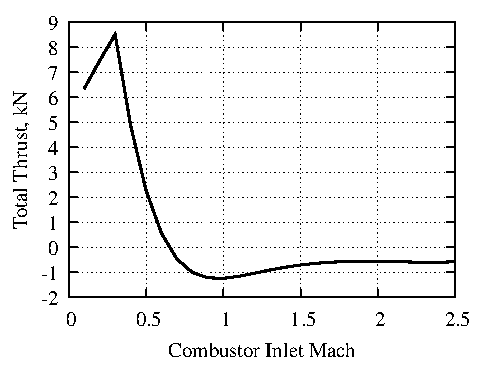
\includegraphics[]{media/performance_parameter_files/part_h_T.pdf}
    \caption{\label{fig:partht}Total Thrust vs \texorpdfstring{\textit{$M_2$}}{M2}}
\end{figure}
The

\subsubsection{Thrust Specific Fuel Consumption}
The

\begin{figure}[H] % Part H: TSFC for varied combustor Mach
    \centering
    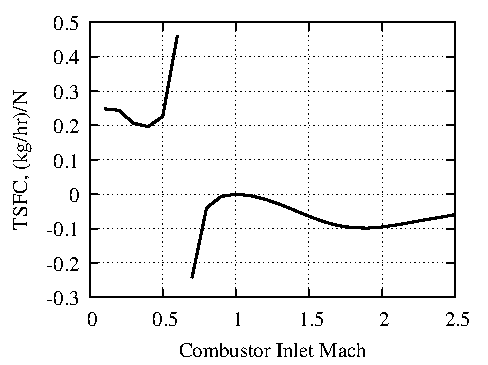
\includegraphics[]{media/performance_parameter_files/part_h_TSFC.pdf}
    \caption{\label{fig:parthtsfc}TSFC vs \texorpdfstring{\textit{$M_2$}}{M2}}
\end{figure}
The

\subsection{Optimized Ram/Scramjet Propulsion System} % Part I
The

\begin{figure}[H] % Part I: propulsion design optimize total thrust
    \centering
    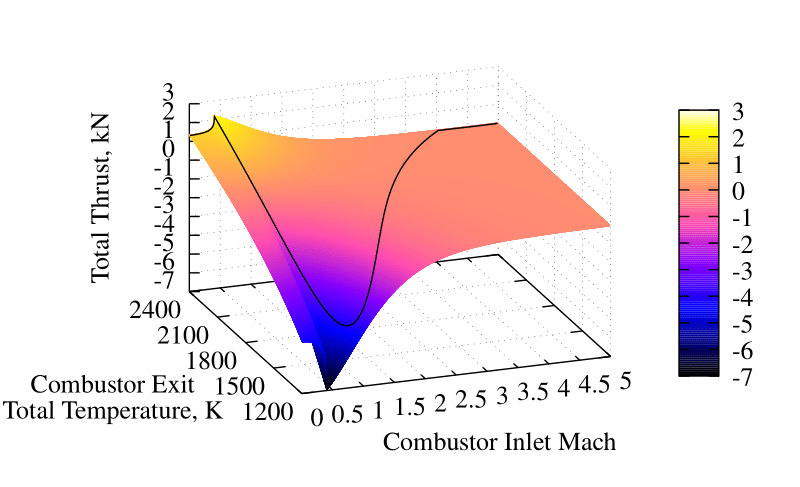
\includegraphics[]{media/propulsion_design_files/total_thrust_plot.pdf}
    \caption{\label{fig:partithrust}Total Thrust}
\end{figure}
The

\begin{figure}[H] % Part I: propulsion design optimize overall efficiency
    \centering
    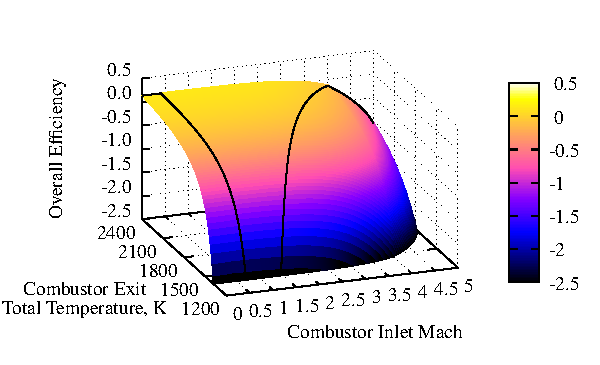
\includegraphics[]{media/propulsion_design_files/eta_o_plot.pdf}
    \caption{\label{fig:partietao}Overall Efficiency}
\end{figure}
The

\begin{table}[H] % Part I: table of optimal hypersonic ram/scramjet parameters
    \caption{\label{tab:design_propsys}Optimal Ram/Scramjet Parameters}
    \centering
    \begin{tabular}{lcccc}
        \hline
            \multirow{2}{*}{Optimizing Parameters}& \multicolumn{4}{c}{Ram/Scramjet Properties}\\
            & $M_2$& $T_{t3}(K)$& $T_{total}(N)$& $\eta_o$\\\hline
            Positive Total Thrust& 0.405& 2400& 2166.102& 0.1308\\
            Overall Efficiency& 0.405& 2400& 2166.102& 0.1308\\
        \hline
    \end{tabular}
\end{table}

\begin{figure}[H] % Part I: propulsion design T-s diagram
    \centering
    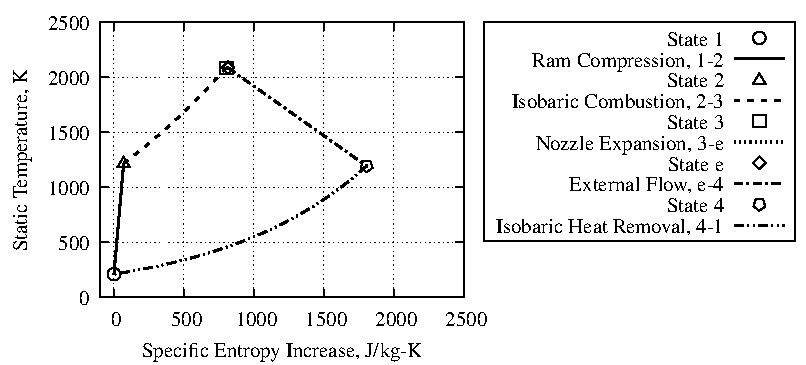
\includegraphics[]{media/ts_plot_files/TS_plot_for_design.pdf}
    \caption{\label{fig:partits}\texorpdfstring{\textit{T-s}}{Ts} Diagram for Chosen Design}
\end{figure}
The


\section{Conclusion}
Although a conclusion may review the main points of the paper, it must not replicate the abstract. A conclusion might elaborate on the importance of the work or suggest applications and extensions. Do not cite references in the conclusion. Note that the conclusion section is the last section of the paper to be numbered. The appendix (if present), funding information, other acknowledgments, and references are listed without numbers.


\section*{Appendix}
\subsection{Tabulated Data}
\begin{table}[H] % Table of Validation Case Inputs
    \caption{\label{tab:val_case_input}Validation Case Inputs}
    \centering
    \begin{tabular}{lcccc}
        \hline
        Name& Variable& Case A& Case B& Units\\\hline
        Flight Altitude& $z$& 4300& 4300& m\\
        Flight Mach Number& $M_1$& 2.4& 2.4\\
        Inlet/Diffuser Efficiency& $\eta_d$& 0.92& 0.92\\
        Combustor Inlet Mach Number& $M_2$& 0.15& 0.4\\
        Combustor Exit Max Allowable Total Temperature& $(T_{t3})_{max}$& 2400& 2400& K\\
        Chosen Fuel Heating Value& $q_f$& 43.2& 43.2& MJ/kg\\
        Nozzle Efficiency& $\eta_n$& 0.94& 0.94\\
        Nozzle Exit Area& $A_e$& 0.015& 0.015& $m^2$\\
        \hline
    \end{tabular}
\end{table}

\begin{longtable}[c]{lcccc} % Table of Validation Case Ouputs
    \caption{\label{tab:val_case_output} Validation Case Outputs}\\
    \hline
    Module& Variable/Property& Case A& Case B& Units\\\hline
    \endfirsthead
    Module 1& $T_1$& 245.9& 245.9& K\\
    & $p_1$& 58.3& 58.3& kPa\\
    & $T_{t1}$& 529.2& 529.2& K\\
    & $p_{t1}$& 851.8& 851.8& kPa\\
    & $c_{p1}$& 1004& 1004& J/(kg-K)\\
    & $a_1$& 314.3& 314.3& m/s\\
    & $V_1$& 754.3& 754.3& m/s\\\hline
    Module 2& $T_{t2}$& 529.2& 529.2& K\\
    & $T_2$& 526.8& 512.8& K\\
    & $p_{t2}$& 730.8& 730.8& kPa\\
    & $p_2$& 719.4& 654.5& kPa\\
    & $c_{p2}$& 1004& 1004& J/(kg-K)\\
    & $a_2$& 460.0& 453.8& m/s\\
    & $V_2$& 69.0& 181.5& m/s\\
    & $\Delta s_{12}$& 43.95& 43.95& J/(kg-K)\\\hline
    Module 3& $T_{t3}$& 2400& 1025& K\\
    & $M_3$& 0.3597& 1.000\\
    & $q_{23}$& 2.34& 0.557& MJ/kg\\
    & $T_3$& 2354& 891& K\\
    & $p_3$& 719.4& 654.5& kPa\\
    & $p_{t3}$& 781.9& 1.200E3& kPa\\
    & $c_{p3}$& 1407& 1146& J/(kg-K)\\
    & $\Delta s_{23}$& 2109& 615& J/(kg-K)\\
    & $\Delta s_{13}$& 2152& 659& J/(kg-K)\\\hline
    Module 4& $M_e$& 1.00& 1.00\\
    & $p_{te}$& 750.0& 1.15E3& kPa\\
    & $p_e$& 409.3& 627.8& kPa\\
    & $T_{te}$& 2400& 1025& K\\
    & $T_e$& 2087& 891& K\\
    & $c_{pe}$& 1360& 1146& J/(kg-K)\\
    & $a_e$& 882& 576& m/s\\
    & $V_e$& 882& 576& m/s\\
    & $\dot{m}_e$& 9.0& 21.2& kg/s\\
    & $\Delta s_{3e}$& 12.0& 12.0& J/(kg-K)\\
    & $\Delta s_{1e}$& 2164& 671& J/(kg-K)\\\hline
    Module 5& $M_4$& 1.90& 2.02\\
    & $p_{t4}$& 379.2& 464.5& kPa\\
    & $p_4$& 58.3& 58.3& kPa\\
    & $T_{t4}$& 2400& 1025& K\\
    & $T_4$& 1558& 635& K\\
    & $c_{p4}$& 1265& 1100& J/(kg-K)\\
    & $a_4$& 762& 486& m/s\\
    & $V_4$& 1447& 985& m/s\\
    & $\Delta s_{e4}$& 195.6& 260& J/(kg-K)\\
    & $\Delta s_{14}$& 2630& 931& J/(kg-K)\\\hline
    Module 6& $\dot{m}_f$& 0.46& 0.27& kg/s\\
    & $\dot{m}_i$& 8.6& 21.0& kg/s\\
    & $f$& 0.054& 0.013\\
    & $T_{jet}$& 1508& -3572& N\\
    & $T_{pressure}$& 5265& 8543& N\\
    & $T_{total}$& 6773& 4971& N\\
    & $V_{eq}$& 1464& 979& m/s\\
    & TSFC& 0.247& 0.196& (kg/hr)/N\\
    & $I_sp$& 1490& 1875& s\\
    & $\eta_{th}$& 0.362& 0.360\\
    & $\eta_p$& 0.680& 0.870\\
    & $\eta_o$& 0.246& 0.312\\
    & $P$& 5.11& 3.75& MW\\
    \hline
\end{longtable}

\subsection{FORTRAN Modules}
\subsubsection{Universal Module Code}
\lstinputlisting[language=FORTRAN,basicstyle=\ttfamily\small]{modules/universal_module.f90}

\subsubsection{Module 1 Code}
\lstinputlisting[language=FORTRAN,basicstyle=\ttfamily\small]{modules/module_1.f90}

\subsubsection{Module 2 Code}
\lstinputlisting[language=FORTRAN,basicstyle=\ttfamily\small]{modules/module_2.f90}

\subsubsection{Module 3 Code}
\lstinputlisting[language=FORTRAN,basicstyle=\ttfamily\small]{modules/module_3.f90}

\subsubsection{Module 4 Code}
\lstinputlisting[language=FORTRAN,basicstyle=\ttfamily\small]{modules/module_4.f90}

\subsubsection{Module 5 Code}
\lstinputlisting[language=FORTRAN,basicstyle=\ttfamily\small]{modules/module_5.f90}

\subsubsection{Module 6 Code}
\lstinputlisting[language=FORTRAN,basicstyle=\ttfamily\small]{modules/module_6.f90}

\subsubsection{Auxiliary Module Code}
\lstinputlisting[language=FORTRAN,basicstyle=\ttfamily\small]{modules/auxiliary_module.f90}


\bibliography{sample}

\end{document}
